\documentclass{article}
\usepackage[UTF8]{ctex} % 用于中文排版
\usepackage{geometry}
\usepackage{indentfirst}
\usepackage{enumitem}

\usepackage{titling}    % 用于自定义标题页
\usepackage{graphicx}
\usepackage{float}

\usepackage{xcolor}
\usepackage{listings}

\usepackage{setspace}

% 页面几何设置
\geometry{a4paper, left=25mm, right=25mm, top=25mm, bottom=25mm}
% 取消首行缩进
\setlength{\parindent}{0pt}
% 行间距设置
\setstretch{1.5}
% 自定义字体大小
\newcommand{\fourhao}{\fontsize{14pt}{\baselineskip}\selectfont} % 四号字体
\newcommand{\xiaosihao}{\fontsize{12pt}{\baselineskip}\selectfont} % 小四号字体
\newcommand{\song}{\CJKfamily{song}}
% 设置代码块格式
\lstset{
    basicstyle = \footnotesize\ttfamily,                 % 设置行距,字体
    numbers = left,                                      % 在左侧显示行号
    numberstyle = \tiny \color{gray},                    % 设定行号格式
    keywordstyle = \bfseries \color[RGB]{40,40,255},     % 设定关键字颜色
    numberstyle = \footnotesize \color{darkgray},           
    commentstyle = \color[RGB]{0,96,96},                 % 设置代码注释的格式
    stringstyle = \color[RGB]{128,0,0},                  % 设置字符串格式
    frame = single,                                      % 不显示背景边框
    backgroundcolor = \color[RGB]{245,245,244},          % 设定背景颜色
    language=Verilog                                     % 设置语言
}
\raggedbottom   % 段落间留白, 避免排版时自动拉伸导致的行间距变化。
\begin{document}

% 封面页面
\begin{titlepage}
    \centering
    \vspace*{2cm}

    \Huge
    \textbf{课程名称:EDA 技术综合设计}

    \vspace{2cm}

    \LARGE
    设计报告名称:设计三\ 二进制转换十进制

    \vspace{4cm}

    \centering
    \Large
    \begin{tabular}{rl}
        班级: & 通信214    \\
        姓名: & \ 王峤宇    \\
        学号: & \ 214022
    \end{tabular}

    \vfill

    \vspace{1cm}
\end{titlepage}

\newpage
% 第一部分
\section*{\fourhao 一、设计内容及原理}
\xiaosihao
\setstretch{1.5}
% 设计项目内容及设计原理,如真值表、状态表及状态转换图、文字说明等。
\subsection*{数码管设计}
利用视觉暂留, 采用动态扫描显示方式完成数码管设计, 每个数码管包括7个LED管和1个小圆点, 
通过8个IO口控制一位数码管显示, 通过分时复用的扫描显示方案进行数码管驱动可以有效地提高
对IO口资源的利用。板上提供的数码管为共阴极数码管。\\
\subsection*{二进制转十进制BCD码}
读取拨码开关输入的二进制后, 通过逐位移位法的方式, 四位二进制数据装换成两个4位的BCD码保存。\\
\subsection*{基础任务}
\textbf{设计任务}:完成4位二进制整数转成十进制数,输入由拨码开关给,输出由数码管显示。\\
\subsection*{提高内容}
\textbf{设计任务}:完成4位二进制纯小数转成十进制数,输入由拨码开关给,输出由数码管显示。\\
小数部分的设计较为困难, 但输入仅有4位二进制, 直接采用case语句完成所有情况的小数输出即可。
\subsection*{拓展任务}
\textbf{任务要求}:完成8位二进制实数转成十进制数(其中四位整数,四位小数),输入由拨码开关给,输出由数码管显示。\\

将前两部分任务设计的模块进行整合, 八位拨码开关, 分别作为四位整数输入和四位小数输入, 数码管两位用于整数输出, 四位用于小数部分输出。\\
\begin{figure}[htbp]
    \centering
    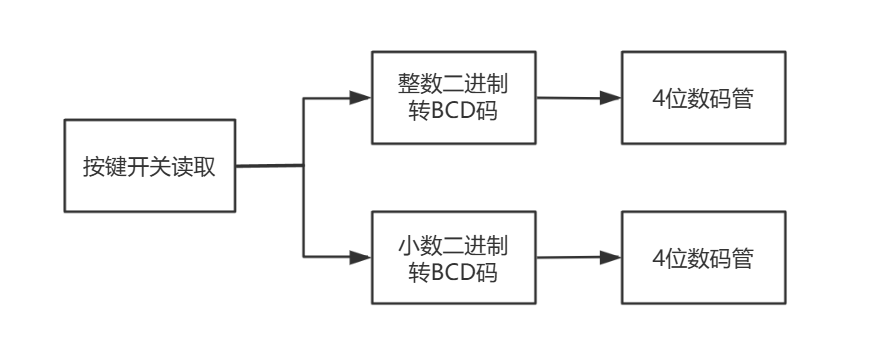
\includegraphics[width=0.4\textwidth]{image/2024-06-28-15-30-37.png}
    \caption{实数二进制转十进制模块框图}
    \label{image_principle_1}
\end{figure}
最终设计得到的8位二进制实数转十进制整数的模块框图如图\ref{image_principle_1}所示。
% 第二部分
\section*{\fourhao 二、设计过程}
\xiaosihao
\setstretch{1.5}
% 从工程建立开始,一直到硬件调试。
% 按照基础任务、提高任务和拓展任务分别给出相应的源文件、仿真文件、约束文件
\subsection*{基础任务}
通过逐位移位法实现的四位无符号数转化为BCD码的源文件如下:
\begin{lstlisting}[language=Verilog, caption={二进制转BCD}]
module int2bcd_4bit(
    input [3:0] uint4,
    output [3:0] outBCD0,
    output [3:0] outBCD1
    );
    reg [11:0] bcd_r0, bcd_r1, bcd_r2;

    /* 直接移位两次 */
    always @(*) begin
        bcd_r0 = {6'b0, uint4, 2'b0};
    end

    /* 移位第三次结果 */
    always @(*) begin
        bcd_r1 = {bcd_r0[10:0], 1'b0};
        if (bcd_r1[7:4] > 4'b0100) bcd_r1[7:4] = bcd_r1[7:4] + 4'b0011;
    end
    
    /* 移位四次结果 */
    always @(*) begin
        bcd_r2 = {bcd_r1[10:0], 1'b0};
    end
    
    /* 输出结果 */
    assign outBCD0 = bcd_r2[7:4];
    assign outBCD1 = bcd_r2[11:8];
endmodule
\end{lstlisting}
时序扫描完成的数码管显示源文件如下, 以四个数码管为单位构建模块:
\begin{lstlisting}[language=Verilog, caption={数码管扫描显示}]
module scan_led_hex_disp_4(
    input clk, rst,         /* 100MHz时钟与复位 */
    input [3:0] hex0, hex1, hex2, hex3, /* 显存 */
    input [3:0] dp,         /* 小数点 */
    output reg [3:0] an,    /* 片选信号 */
    output reg [7:0] sseg   /* 八段数码管接口 */
    );

    localparam N = 16 + 2;  /* 100MHz时钟分频, 100Mhz/ 2^16 */         
    reg [N-1:0] regN;

    always @(posedge clk, posedge rst) begin
        if (rst)            /* 异步, 高电平复位 */
            regN <= 0;
        else 
            regN <= regN + 1;
    end

    always @(*) begin       /* 时分复用 */
        case (regN[N-1:N-2])
            2'b00: begin
                an <= 4'b0001;
                sseg[6:0] <= dt_translate(hex0);
                sseg[7] <= dp[3];
            end
            2'b01: begin
                an <= 4'b0010;
                sseg[6:0] <= dt_translate(hex1);
                sseg[7] <= dp[2];
            end
            2'b10: begin
                an <= 4'b0100;
                sseg[6:0] <= dt_translate(hex2);
                sseg[7] <= dp[1];
            end
            2'b11: begin
                an <= 4'b1000;
                sseg[6:0] <= dt_translate(hex3);
                sseg[7] <= dp[0];
            end 
        endcase
    end

    function [6:0] dt_translate;    /* 数码管译码函数 */
        input [3:0] data;
        begin
            case(data)
                4'd0: dt_translate = 7'b1111110;     //number 0 -> 0x7e
                4'd1: dt_translate = 7'b0110000;     //number 1 -> 0x30
                4'd2: dt_translate = 7'b1101101;     //number 2 -> 0x6d
                4'd3: dt_translate = 7'b1111001;     //number 3 -> 0x79
                4'd4: dt_translate = 7'b0110011;     //number 4 -> 0x33
                4'd5: dt_translate = 7'b1011011;     //number 5 -> 0x5b
                4'd6: dt_translate = 7'b1011111;     //number 6 -> 0x5f
                4'd7: dt_translate = 7'b1110000;     //number 7 -> 0x70
                4'd8: dt_translate = 7'b1111111;     //number 8 -> 0x7f
                4'd9: dt_translate = 7'b1111011;     //number 9 -> 0x7b
            endcase
        end
    endfunction
endmodule
\end{lstlisting}
整体系统的top文件如下:
\begin{lstlisting}[language=Verilog, caption={top文件}]
module bin2dec_top(
    input clk,                  /* 100MHz */
    input rst,                  /* 高电平异步复位 */
    input [7:0] real_bin,       /* 输入的四位整数加四位小数的二进制实数 */
    output [7:0] sseg1, sseg2,  /* 八段数码管 */
    output [3:0] an1, an2       /* 片选信号 */
    );

    /* 计算整数部分的BCD码 */
    wire [3:0] bcd_int0, bcd_int1;
    int2bcd_4bit  int2bcd_4bit_inst (
        .uint4(real_bin[7:4]),
        .outBCD0(bcd_int0),
        .outBCD1(bcd_int1)
    );

    /* 第一个四数码管显示整数部分 */
    scan_led_hex_disp_4  scan_led_hex_disp_4_inst_0 (
        .clk(clk), .rst(rst),
        .hex0(4'b0000), .hex1(4'b0000), .hex2(bcd_int1), .hex3(bcd_int0), .dp(4'b0001),
        .an(an1), .sseg(sseg1)
    );

    scan_led_hex_disp_4  scan_led_hex_disp_4_inst_1 (
        .clk(clk), .rst(rst),
        .hex0(4'b0000), .hex1(4'b0000), .hex2(4'b0000), .hex3(4'b0000), .dp(4'b0000),
        .an(an2), .sseg(sseg2)
    );
endmodule
\end{lstlisting}
仿真文件如下:
\begin{lstlisting}[language=Verilog, caption={整数部分仿真文件}]
module bin2dec_top_tb;
    reg  clk;
    reg  rst;
    reg [7:0] real_bin;
    wire [7:0] sseg1, sseg2;
    wire [3:0] an1, an2;

    initial begin
        clk = 0;
        rst = 1;
        #10;
        clk = 1;
        #10;
        rst = 0;
        real_bin = 8'b0;
        forever begin
            #100;
            real_bin = real_bin + 8'b0001_0000;
            if (real_bin == 8'b0) begin
                $finish;
            end  
        end
    end
    /* 生成时钟 */
    always @(*) #5 clk <= ~clk;
    /* 例化top */
    bin2dec_top  bin2dec_top_inst (
        .clk(clk),
        .rst(rst),
        .real_bin(real_bin),
        .sseg1(sseg1),
        .sseg2(sseg2),
        .an1(an1),
        .an2(an2)
    );
endmodule
\end{lstlisting}
\subsection*{提高任务}
浮点数设计较为复杂, 但由于输入位数较少, 通过case语句实现, 实现源文件如下:
\begin{lstlisting}[language=Verilog, caption={二进制小数转十进制}]
module float2bcd_4bit(
    input [3:0] float4,
    output [3:0] BCD0, BCD1, BCD2, BCD3
    );
    reg [3:0] BCD0_r, BCD1_r, BCD2_r, BCD3_r;

    always @(*) begin
        case (float4)
            4'b0000: {BCD0_r, BCD1_r, BCD2_r, BCD3_r} = 16'b0;                    // 0.0000
            4'b0001: {BCD0_r, BCD1_r, BCD2_r, BCD3_r} = {4'd0, 4'd6, 4'd2, 4'd5}; // 0.0625
            4'b0010: {BCD0_r, BCD1_r, BCD2_r, BCD3_r} = {4'd1, 4'd2, 4'd5, 4'd0}; // 0.125
            4'b0011: {BCD0_r, BCD1_r, BCD2_r, BCD3_r} = {4'd1, 4'd8, 4'd7, 4'd5}; // 0.1875
            4'b0100: {BCD0_r, BCD1_r, BCD2_r, BCD3_r} = {4'd2, 4'd5, 4'd0, 4'd0}; // 0.25
            4'b0101: {BCD0_r, BCD1_r, BCD2_r, BCD3_r} = {4'd3, 4'd1, 4'd2, 4'd5}; // 0.3125
            4'b0110: {BCD0_r, BCD1_r, BCD2_r, BCD3_r} = {4'd3, 4'd7, 4'd5, 4'd0}; // 0.375
            4'b0111: {BCD0_r, BCD1_r, BCD2_r, BCD3_r} = {4'd4, 4'd3, 4'd7, 4'd5}; // 0.4375
            4'b1000: {BCD0_r, BCD1_r, BCD2_r, BCD3_r} = {4'd5, 4'd0, 4'd0, 4'd0}; // 0.5
            4'b1001: {BCD0_r, BCD1_r, BCD2_r, BCD3_r} = {4'd5, 4'd6, 4'd2, 4'd5}; // 0.5625
            4'b1010: {BCD0_r, BCD1_r, BCD2_r, BCD3_r} = {4'd6, 4'd2, 4'd5, 4'd0}; // 0.625
            4'b1011: {BCD0_r, BCD1_r, BCD2_r, BCD3_r} = {4'd6, 4'd8, 4'd7, 4'd5}; // 0.6875
            4'b1100: {BCD0_r, BCD1_r, BCD2_r, BCD3_r} = {4'd7, 4'd5, 4'd0, 4'd0}; // 0.75
            4'b1101: {BCD0_r, BCD1_r, BCD2_r, BCD3_r} = {4'd8, 4'd1, 4'd2, 4'd5}; // 0.8125
            4'b1110: {BCD0_r, BCD1_r, BCD2_r, BCD3_r} = {4'd8, 4'd7, 4'd5, 4'd0}; // 0.875
            4'b1111: {BCD0_r, BCD1_r, BCD2_r, BCD3_r} = {4'd9, 4'd3, 4'd7, 4'd5}; // 0.9375
            default: {BCD0_r, BCD1_r, BCD2_r, BCD3_r} = {4'd0, 4'd0, 4'd0, 4'd0}; // Default case
        endcase    
    end

    assign BCD0 = BCD0_r;
    assign BCD1 = BCD1_r;
    assign BCD2 = BCD2_r;
    assign BCD3 = BCD3_r;
endmodule
\end{lstlisting}
修改后的top源文件新增内容如下:
\begin{lstlisting}[language=Verilog, caption={添加小数部分的Top文件修改内容}]
/* 计算小数部分的BCD码 */
wire [3:0] bcd_float0, bcd_float1, bcd_float2, bcd_float3;
float2bcd_4bit  float2bcd_4bit_inst (
    .float4(real_bin[3:0]),
    .BCD0(bcd_float0), .BCD1(bcd_float1),
    .BCD2(bcd_float2), .BCD3(bcd_float3)
);
scan_led_hex_disp_4  scan_led_hex_disp_4_inst_1 (
    .clk(clk), .rst(rst),
    .hex0(bcd_float0), .hex1(bcd_float1), .hex2(bcd_float2), .hex3(bcd_float3), .dp(4'b0000),
    .an(an2), .sseg(sseg2)
);
\end{lstlisting}
对应的仿真文件的更改部分如下, 将激励改为遍历小数部分测试, 并且不再对数码管输出进行仿真测试, 直接测试小数输出bcd是否正确:
\begin{lstlisting}[language=Verilog, caption={小数转十进制仿真文件}]
initial begin
    clk = 0;
    rst = 1;
    #10;
    clk = 1;
    #10;
    rst = 0;
    real_bin = 8'b0;
    forever begin
        #100;
        real_bin = real_bin + 8'b0000_0001; /* 遍历浮点数情况 */
        if (real_bin[3:0] == 4'b0) begin    
            $finish;
        end
    end
end
\end{lstlisting}
\subsection*{拓展任务}
模块整合后的源文件如下:
\begin{lstlisting}[language=Verilog, caption={最终top源文件}]
module bin2dec_top(
    input clk,                  /* 100MHz */
    input rst,                  /* 高电平异步复位 */
    input [7:0] real_bin,       /* 输入的四位整数加四位小数的二进制实数 */
    output [7:0] sseg1, sseg2,  /* 八段数码管 */
    output [3:0] an1, an2       /* 片选信号 */
    );

    /* 计算整数部分的BCD码 */
    wire [3:0] bcd_int0, bcd_int1;
    int2bcd_4bit  int2bcd_4bit_inst (
        .uint4(real_bin[7:4]),
        .outBCD0(bcd_int0),
        .outBCD1(bcd_int1)
    );

    /* 第一个四数码管显示整数部分 */
    scan_led_hex_disp_4  scan_led_hex_disp_4_inst_0 (
        .clk(clk), .rst(rst),
        .hex0(4'b0000), .hex1(4'b0000), .hex2(bcd_int1), .hex3(bcd_int0), .dp(4'b0001),
        .an(an1), .sseg(sseg1)
    );

    /* 计算小数部分的BCD码 */
    wire [3:0] bcd_float0, bcd_float1, bcd_float2, bcd_float3;
    float2bcd_4bit  float2bcd_4bit_inst (
        .float4(real_bin[3:0]),
        .BCD0(bcd_float0), .BCD1(bcd_float1),
        .BCD2(bcd_float2), .BCD3(bcd_float3)
    );
    scan_led_hex_disp_4  scan_led_hex_disp_4_inst_1 (
        .clk(clk), .rst(rst),
        .hex0(bcd_float0), .hex1(bcd_float1), .hex2(bcd_float2), .hex3(bcd_float3), .dp(4'b0000),
        .an(an2), .sseg(sseg2)
    );
endmodule
\end{lstlisting}
仿真文件中的更改后的激励如下, 实现对所有可能输入数据的遍历:
\begin{lstlisting}[language=Verilog, caption={系统仿真激励}]
initial begin
    clk = 0;
    rst = 1;
    #10;
    clk = 1;
    #10;
    rst = 0;
    real_bin = 8'b0;
    forever begin
        #100;
        real_bin = real_bin + 8'b0000_0001; /* 遍历浮点数情况 */
        if (real_bin == 8'b0) begin
            $finish;
        end
    end
end
\end{lstlisting}
本系统设计最终需要用到, 八个数码管, 其中数码管为共阴极, 由三极管驱动, 整个系统的约束文件下:
\begin{lstlisting}[language=Verilog, caption={系统约束文件}]
set_property IOSTANDARD LVCMOS33 [get_ports clk]
set_property IOSTANDARD LVCMOS33 [get_ports rst]
set_property PACKAGE_PIN P17 [get_ports clk]
set_property PACKAGE_PIN R11 [get_ports rst]
set_property IOSTANDARD LVCMOS33 [get_ports {real_bin[7]}]
set_property IOSTANDARD LVCMOS33 [get_ports {real_bin[6]}]
set_property IOSTANDARD LVCMOS33 [get_ports {real_bin[5]}]
set_property IOSTANDARD LVCMOS33 [get_ports {real_bin[4]}]
set_property IOSTANDARD LVCMOS33 [get_ports {real_bin[3]}]
set_property IOSTANDARD LVCMOS33 [get_ports {real_bin[2]}]
set_property IOSTANDARD LVCMOS33 [get_ports {real_bin[1]}]
set_property IOSTANDARD LVCMOS33 [get_ports {real_bin[0]}]
set_property IOSTANDARD LVCMOS33 [get_ports {sseg1[7]}]
set_property IOSTANDARD LVCMOS33 [get_ports {sseg1[6]}]
set_property IOSTANDARD LVCMOS33 [get_ports {sseg1[5]}]
set_property IOSTANDARD LVCMOS33 [get_ports {sseg1[4]}]
set_property IOSTANDARD LVCMOS33 [get_ports {sseg1[3]}]
set_property IOSTANDARD LVCMOS33 [get_ports {sseg1[2]}]
set_property IOSTANDARD LVCMOS33 [get_ports {sseg1[1]}]
set_property IOSTANDARD LVCMOS33 [get_ports {sseg1[0]}]
set_property IOSTANDARD LVCMOS33 [get_ports {sseg2[7]}]
set_property IOSTANDARD LVCMOS33 [get_ports {sseg2[6]}]
set_property IOSTANDARD LVCMOS33 [get_ports {sseg2[5]}]
set_property IOSTANDARD LVCMOS33 [get_ports {sseg2[4]}]
set_property IOSTANDARD LVCMOS33 [get_ports {sseg2[3]}]
set_property IOSTANDARD LVCMOS33 [get_ports {sseg2[2]}]
set_property IOSTANDARD LVCMOS33 [get_ports {sseg2[1]}]
set_property IOSTANDARD LVCMOS33 [get_ports {sseg2[0]}]
set_property IOSTANDARD LVCMOS33 [get_ports {an1[3]}]
set_property IOSTANDARD LVCMOS33 [get_ports {an1[2]}]
set_property IOSTANDARD LVCMOS33 [get_ports {an1[1]}]
set_property IOSTANDARD LVCMOS33 [get_ports {an1[0]}]
set_property IOSTANDARD LVCMOS33 [get_ports {an2[3]}]
set_property IOSTANDARD LVCMOS33 [get_ports {an2[2]}]
set_property IOSTANDARD LVCMOS33 [get_ports {an2[1]}]
set_property IOSTANDARD LVCMOS33 [get_ports {an2[0]}]
set_property PACKAGE_PIN P5 [get_ports {real_bin[7]}]
set_property PACKAGE_PIN P4 [get_ports {real_bin[6]}]
set_property PACKAGE_PIN P3 [get_ports {real_bin[5]}]
set_property PACKAGE_PIN P2 [get_ports {real_bin[4]}]
set_property PACKAGE_PIN R2 [get_ports {real_bin[3]}]
set_property PACKAGE_PIN M4 [get_ports {real_bin[2]}]
set_property PACKAGE_PIN N4 [get_ports {real_bin[1]}]
set_property PACKAGE_PIN R1 [get_ports {real_bin[0]}]
set_property PACKAGE_PIN G2 [get_ports {an1[0]}]
set_property PACKAGE_PIN C2 [get_ports {an1[1]}]
set_property PACKAGE_PIN C1 [get_ports {an1[2]}]
set_property PACKAGE_PIN H1 [get_ports {an1[3]}]
set_property PACKAGE_PIN G6 [get_ports {an2[3]}]
set_property PACKAGE_PIN E1 [get_ports {an2[2]}]
set_property PACKAGE_PIN F1 [get_ports {an2[1]}]
set_property PACKAGE_PIN G1 [get_ports {an2[0]}]
set_property PACKAGE_PIN D5 [get_ports {sseg1[7]}]
set_property PACKAGE_PIN B4 [get_ports {sseg1[6]}]
set_property PACKAGE_PIN A4 [get_ports {sseg1[5]}]
set_property PACKAGE_PIN A3 [get_ports {sseg1[4]}]
set_property PACKAGE_PIN B1 [get_ports {sseg1[3]}]
set_property PACKAGE_PIN A1 [get_ports {sseg1[2]}]
set_property PACKAGE_PIN B3 [get_ports {sseg1[1]}]
set_property PACKAGE_PIN B2 [get_ports {sseg1[0]}]
set_property PACKAGE_PIN H2 [get_ports {sseg2[7]}]
set_property PACKAGE_PIN D4 [get_ports {sseg2[6]}]
set_property PACKAGE_PIN E3 [get_ports {sseg2[5]}]
set_property PACKAGE_PIN D3 [get_ports {sseg2[4]}]
set_property PACKAGE_PIN F4 [get_ports {sseg2[3]}]
set_property PACKAGE_PIN F3 [get_ports {sseg2[2]}]
set_property PACKAGE_PIN E2 [get_ports {sseg2[1]}]
set_property PACKAGE_PIN D2 [get_ports {sseg2[0]}]
\end{lstlisting}
% 第三部分
\section*{\fourhao 三、仿真结果}
\xiaosihao
\setstretch{1.5}
% 对仿真图像要有解释,要对所有的可能性进行标注及解释
% 按照基础任务、提高任务和拓展任务分别给出仿真结果
\subsection*{基础任务}
\begin{figure}[H]
    \centering
    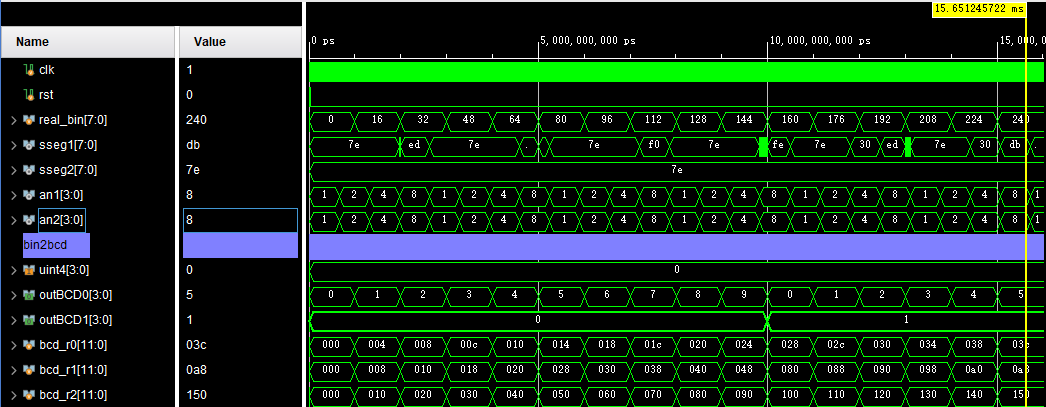
\includegraphics[width=0.7\textwidth]{image/2024-06-16-19-26-59.png}
    \caption{整数部分仿真结果}
    \label{image_int_sim}
\end{figure}
对整数部分和数码管显示的仿真如图\ref{image_int_sim}所示, 仿真文件中控制每1ms控制输入的实数数据自增, 整数部分从0自增到15, 相应的BCD码输出正确。
显示部分扫描四个数码管的片选步进为100MHz的2\^16分频, 大概在1.5KHz左右, 0.6ms。可以通过时序图看到随着片选信号的改变, 数码管的输出也在随着改变。
\subsection*{提高任务}
\begin{figure}[H]
    \centering
    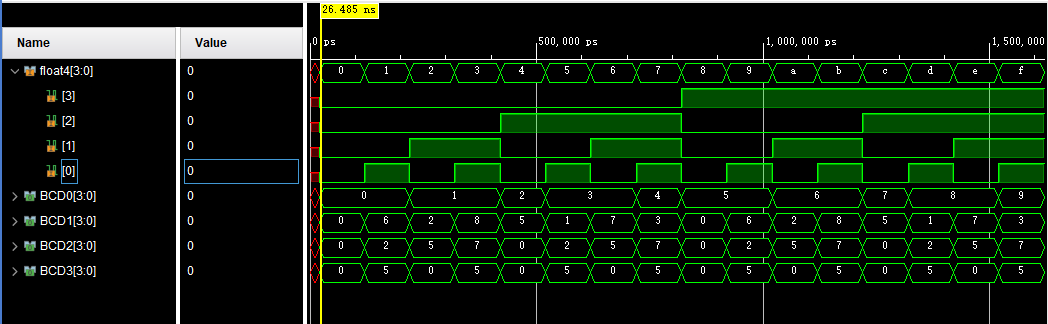
\includegraphics[width=0.7\textwidth]{image/2024-06-16-20-44-36.png}
    \caption{小数部分仿真结果}
    \label{image_float_sim}
\end{figure}
对小数部分的仿真如图\ref{image_int_sim}所示, 仿真文件中控制每100ns控制输入的实数小数部分数据自增, 小数部分的数据从0000到1111, 对应数据从0000到0.9375, 
对应仿真图中数据为16进制显示, 可以看到对应的4个BCD码从0000增加到9375, 对小数部分的BCD码解析输出无误。
\subsection*{拓展任务}
\begin{figure}[htbp]
    \centering
    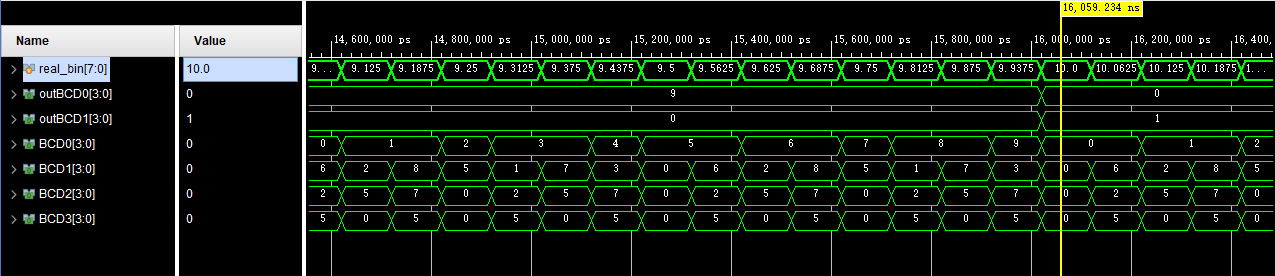
\includegraphics[width=0.7\textwidth]{image/2024-06-16-22-06-07.png}
    \caption{实数设计仿真结果}
    \label{image_real_sim}
\end{figure}
对最终的实数设计的仿真如图\ref{image_real_sim}所示, 仿真文件中控制每100ns控制输入的实数数据自增, 每次增加0.0625,实数的数据从00000000到11111111, 对应数据从0到15.9375, 
对应仿真图中数据输入实数改为小数模式, 由于仿真窗口限制, 仅展示部分结果, 可以看到对应的十进制小数(二进制存储状态)被转化成六个BCD码, 并一一对应, 准确无误。
% 第四部分
\section*{\fourhao 四、硬件验证结果}
\xiaosihao
\setstretch{1.5}
% 记录加编程器与拨码开关和发光二极管、数码管等的连接情况。记录开发板硬件验证结果,并分析其结果的正确性。
% 按照基础任务、提高任务和拓展任务分别分析
\subsection*{基础任务}
\begin{figure}[H]
    \centering
    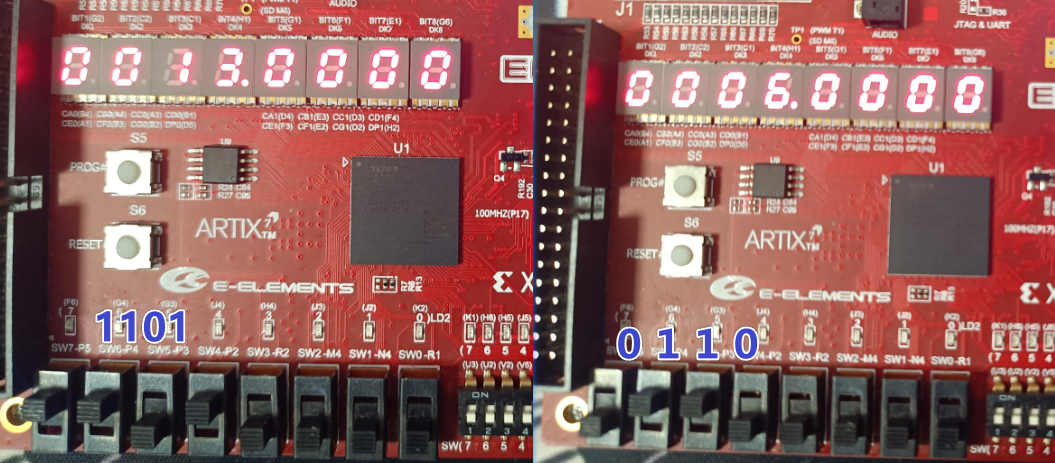
\includegraphics[width=0.7\textwidth]{image/2024-06-16-20-19-02.png}
    \caption{整数部分硬件验证}
    \label{image_int_hardware}
\end{figure}
针对整数部分的数码管的二进制转十进制硬件验证结果如图\ref{image_int_hardware}所示, 其中拨码开关从左开始数的高四位作为整数部分的输出, 
由图中标注可以得到, 当输入为4'b1101时, 对应的十进制数是13, 显示成功, 并且显示由小数点用于区分整数和小数。
\subsection*{提高任务}
\begin{figure}[H]
    \centering
    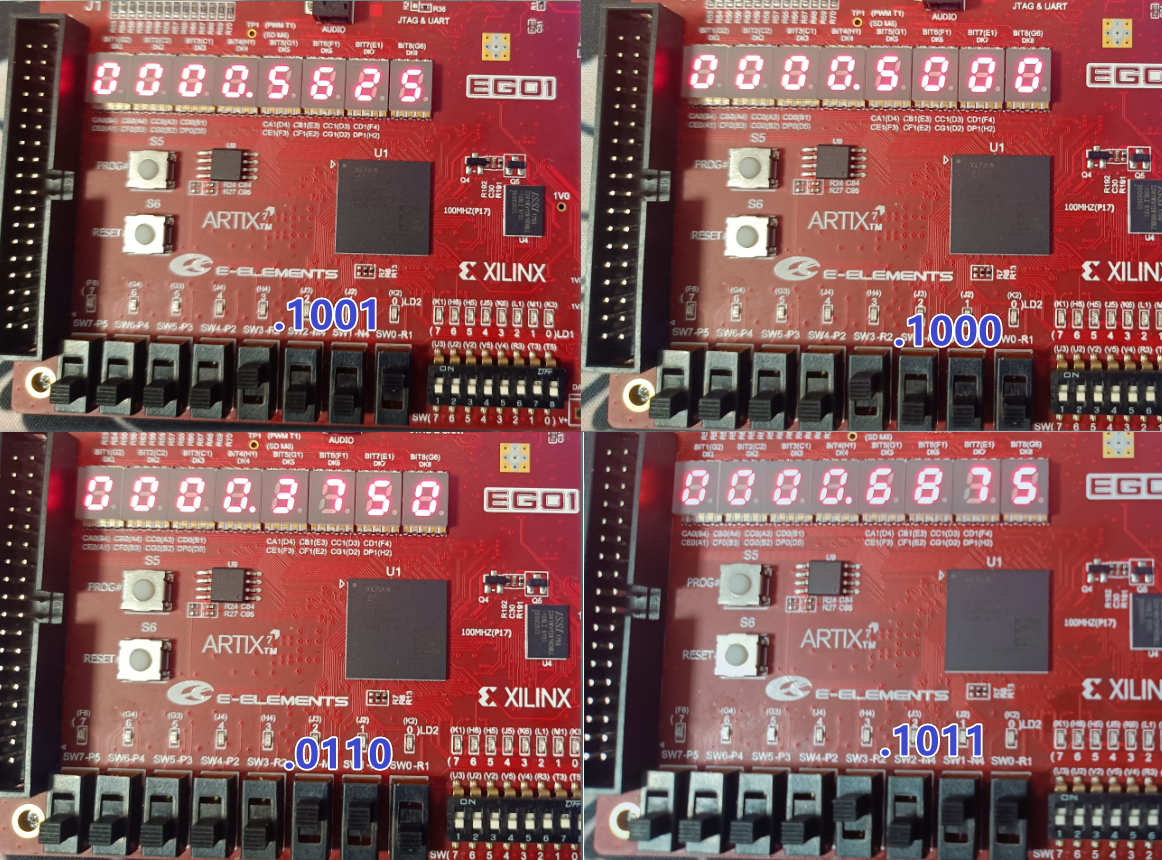
\includegraphics[width=0.6\textwidth]{image/2024-06-16-21-42-54.png}
    \caption{小数部分硬件验证}
    \label{image_float_hardware}
\end{figure}
针对小数部分的数码管的二进制转十进制硬件验证结果如图\ref{image_float_hardware}所示, 其中拨码开关从左开始数的后四个作为二进制小数部分的输入, 
由图中标注可以得到, 当输入为.1001时, 输出的十进制小数部分为.5625, .0110时输出为.3750, 以.0110为例, 输出为
$$.0110: 0*2^{-1} + 1*2^{-2} + 1*2^{-3} + 0*2^{-4} = 0.3750$$
\subsection*{拓展任务}
\begin{figure}[H]
    \centering
    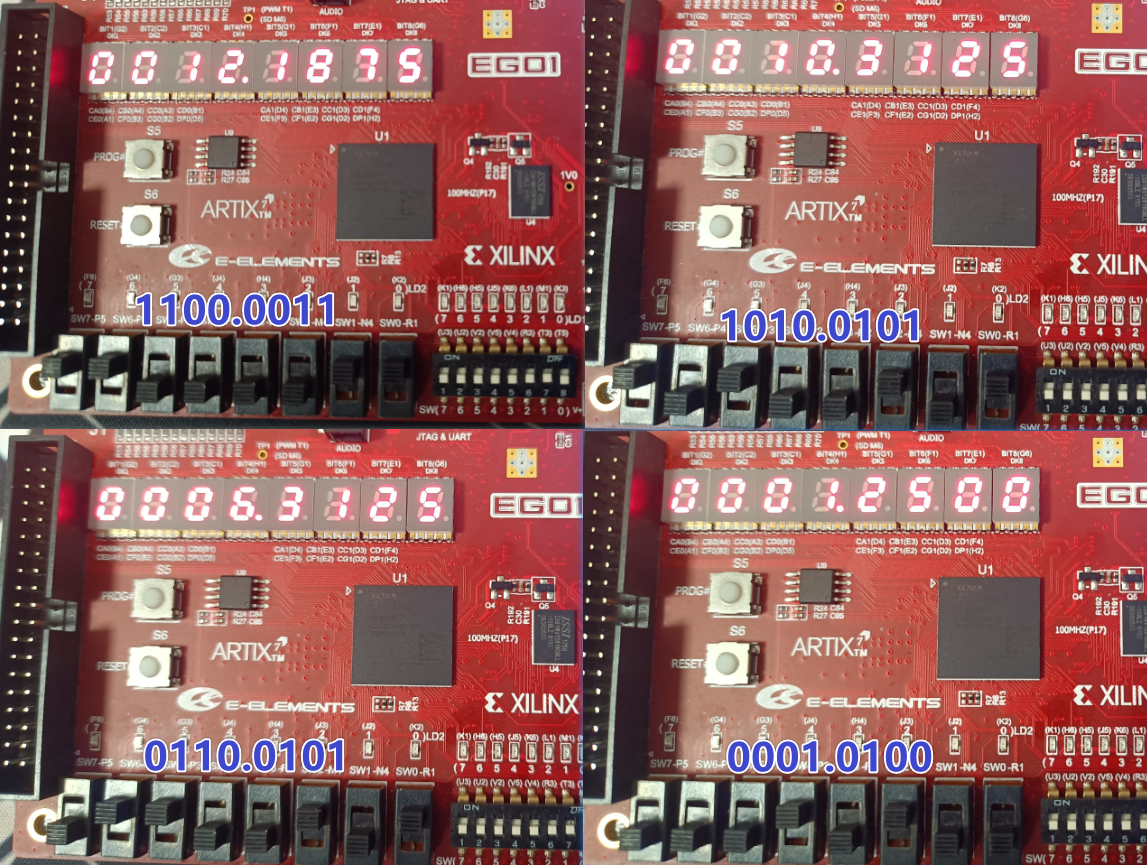
\includegraphics[width=0.7\textwidth]{image/2024-06-16-22-29-35.png}
    \caption{八位实数硬件验证}
    \label{image_real_hardware}
\end{figure}
针对小数部分的数码管的二进制转十进制硬件验证结果如图\ref{image_real_hardware}所示。
% 第五部分
\section*{\fourhao 五、问题解决}
\xiaosihao
\setstretch{1.5}
% 设计过程中遇到的问题及解决的方法。
\subsection*{设计初期, 对二进制转十进制的硬件实现思路不了解}
解决: 通过查阅资料, 了解了二进制码转BCD码的逐位移位法, 并且在设计过程中对四位的逐位移位计算过程进行了一定的优化, 可以得到结论, 
对于四位二进制转化为BCD码的过程中, 仅需要一次判断大四加三即可, 通过wire实现级间缓冲, 利用组合逻辑描述实现类似时序逻辑数据处理的效果。
\subsection*{在设计组合逻辑的时候assign语句难以实现复杂逻辑描述}
解决: 对于wire等线网类型数据, 无法在always语句块中赋值, 无法直接使用if或者case等条件分支语句块, 只能使用简单的问号表达式, 
通常在实现复杂组合逻辑时可以先声明相应的reg类型变量, 在always语句块中完成组合逻辑设计, 最后再通过assign语句将相应的reg数据赋值给wire线网类型。
% 第六部分
\section*{\fourhao 六、心得体会}
\xiaosihao
如果不考虑数码管显示的话, 本次实验与实验二同样是进行组合逻辑电路设计, 但可以明显感受到难度的上升, 
本次电路设计过程中, 主要的难点在于二进制整数转化为BCD和二进制小数转化为BCD码的实现, 由于本次设计
过程中,只需要考虑4位二进制的BCD码输出, 其仅仅相当于4位输入的组合逻辑电路, 最终得到的综合工具会对
其优化, 难点主要在于如何用Verilog语句描述该过程, 比如Verilog中循环语句对于二进制转BCD的逐位移位
法很有效, 虽然for循环有着与C语言相同的语法风格, 但for循环并不存在对应的实际电路, 综合工具有可能
会将for的循环体视作一个模块, 然后综合时很有可能生成循环次数个模块, 也有可能通过优化直接将for循环
实现的功能用其他电路替代, 需要谨慎使用。
\end{document}
